\begin{figure}[h]\centering
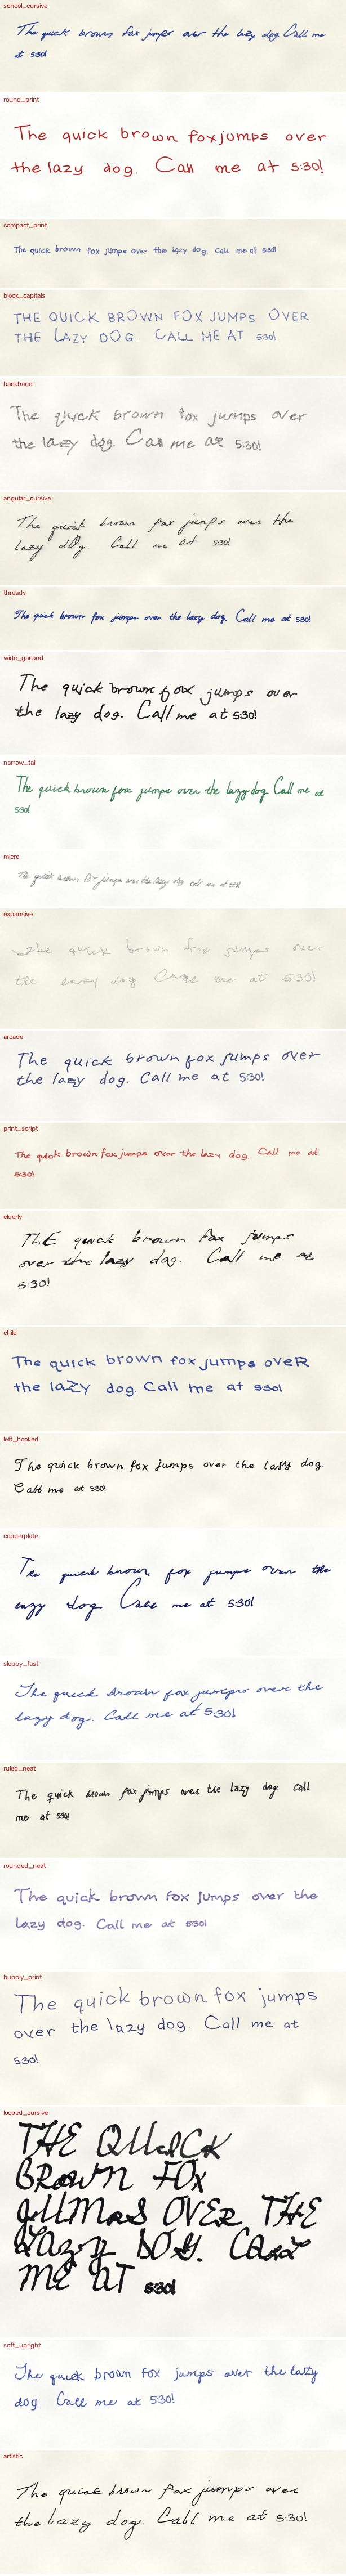
\includegraphics[width=0.95\textwidth,height=0.88\textheight,keepaspectratio]{figs/persons.jpg}
\caption{One individual of each of the 24 types (casual style).}\end{figure}
\clearpage
\begin{figure}[h]\centering
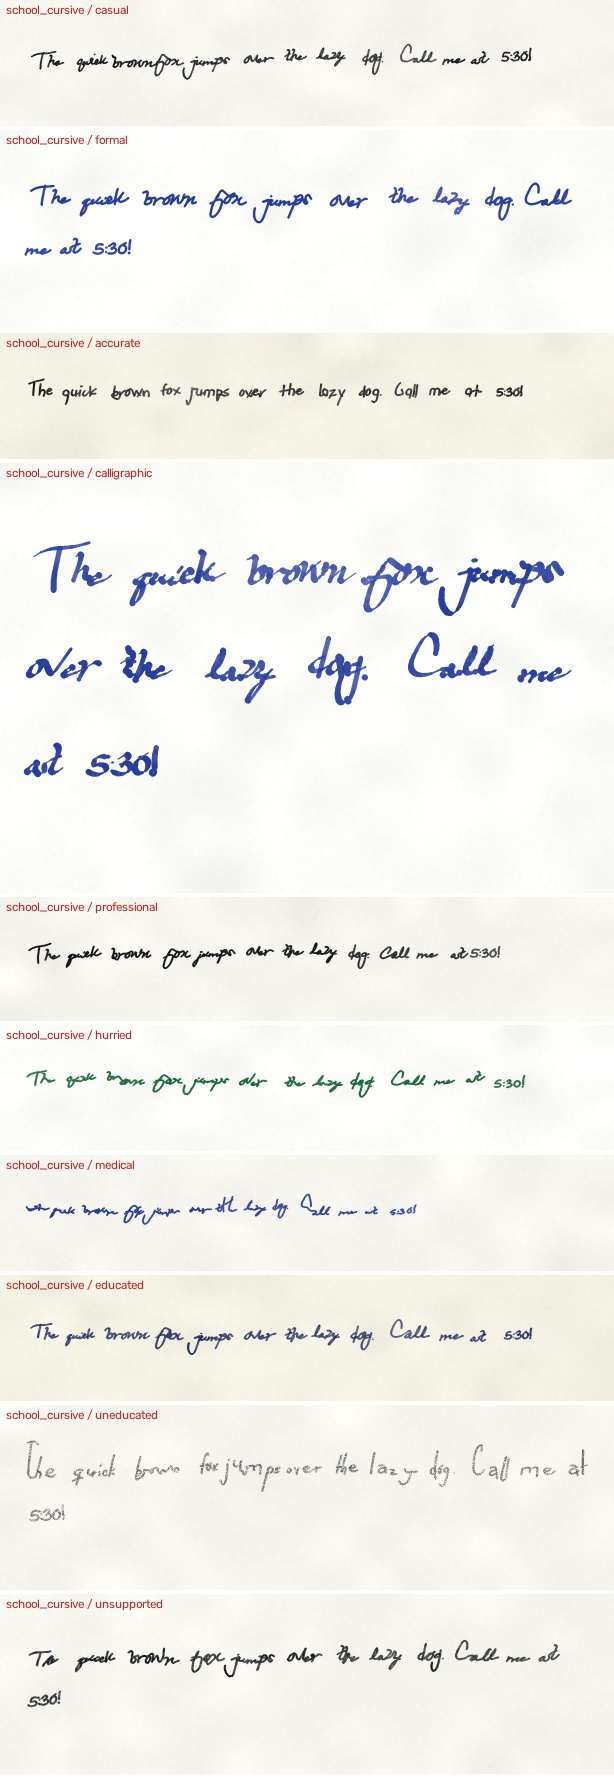
\includegraphics[width=0.95\textwidth,height=0.88\textheight,keepaspectratio]{figs/styles_school_cursive.jpg}
\caption{One school-cursive individual in the 10 styles.}\end{figure}
\clearpage
\begin{figure}[h]\centering
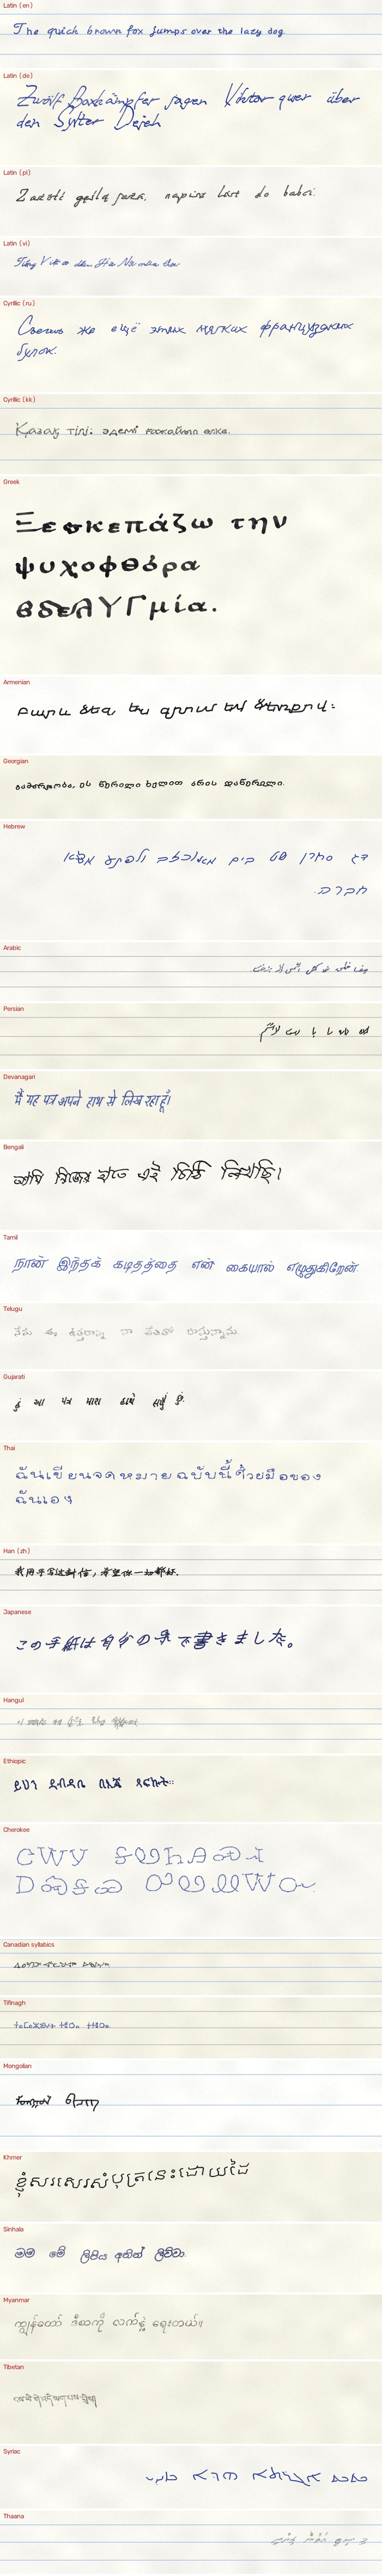
\includegraphics[width=0.95\textwidth,height=0.88\textheight,keepaspectratio]{figs/scripts.jpg}
\caption{Random individuals writing 32 scripts.}\end{figure}
\clearpage
\begin{figure}[h]\centering
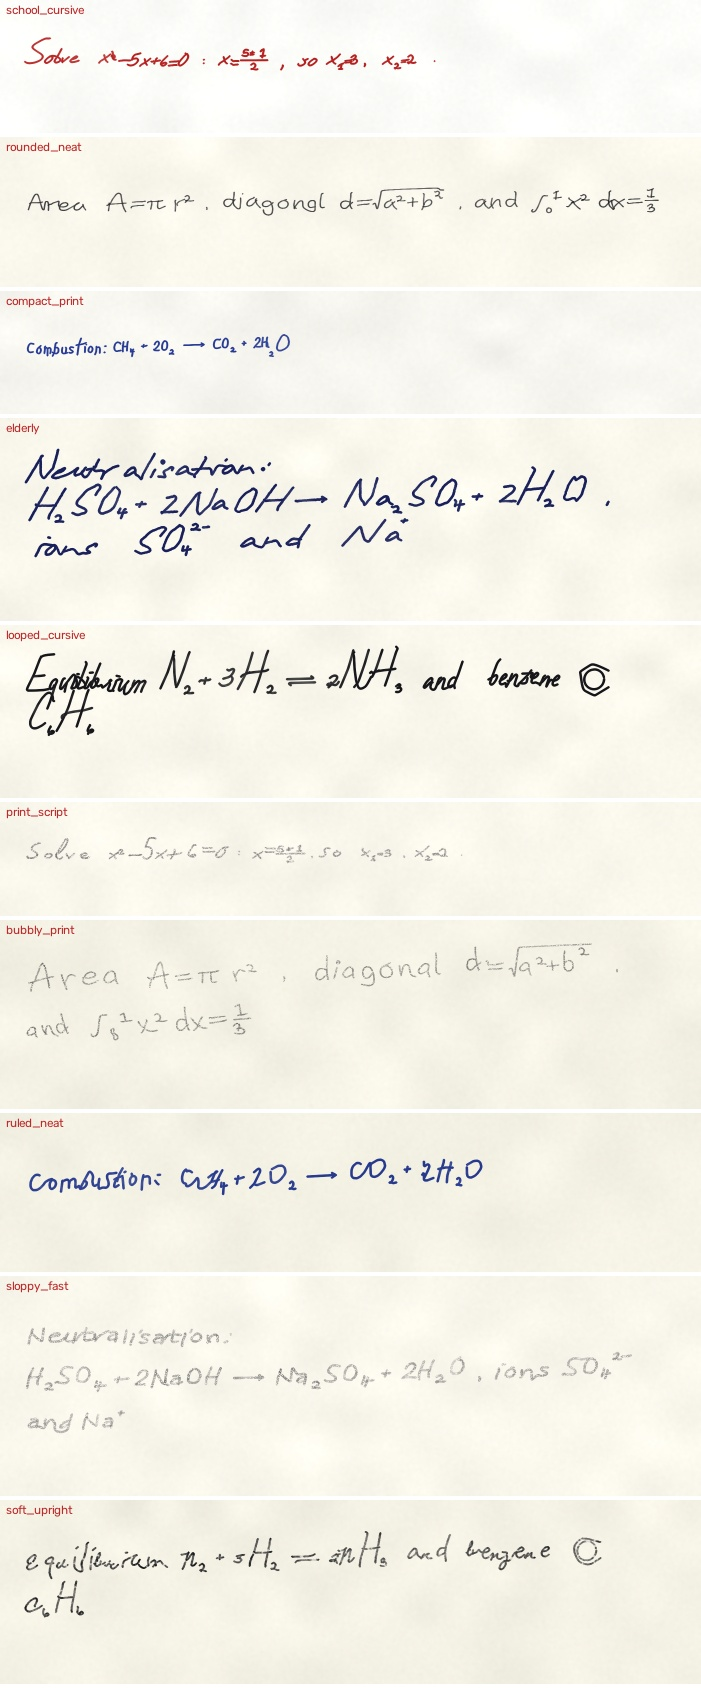
\includegraphics[width=0.95\textwidth,height=0.88\textheight,keepaspectratio]{figs/math_chemistry.jpg}
\caption{Inline mathematics and chemistry.}\end{figure}
\clearpage
\begin{figure}[h]\centering
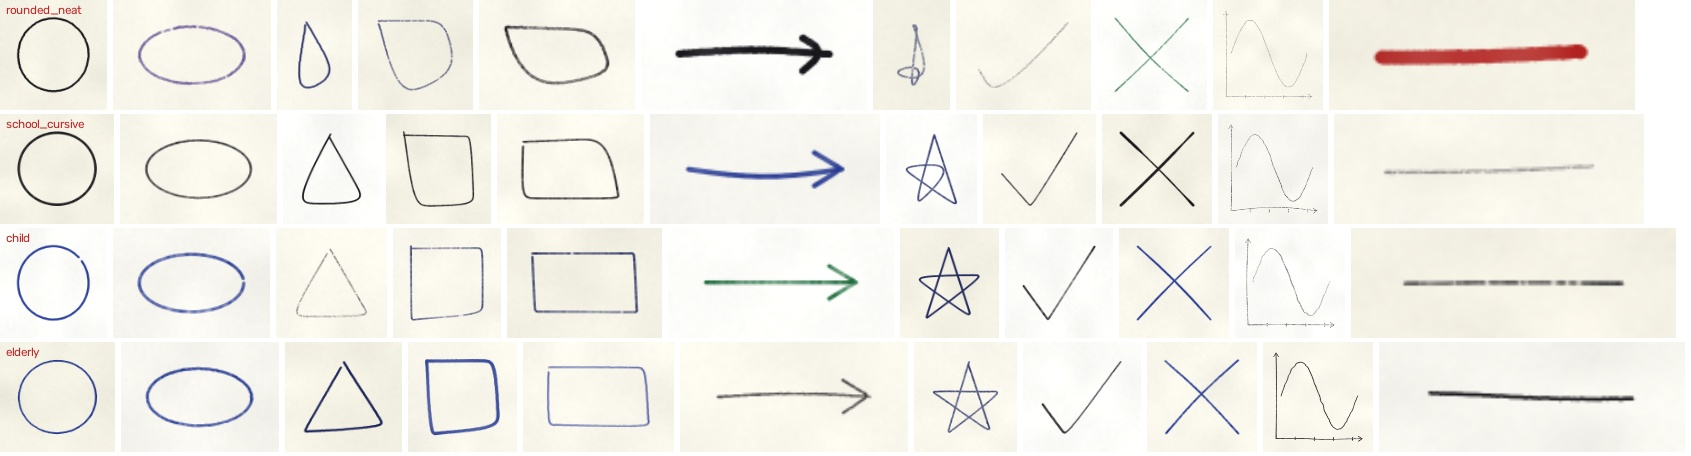
\includegraphics[width=0.95\textwidth,height=0.88\textheight,keepaspectratio]{figs/figures.jpg}
\caption{Hand-drawn figures by four types.}\end{figure}
\clearpage
\begin{figure}[h]\centering
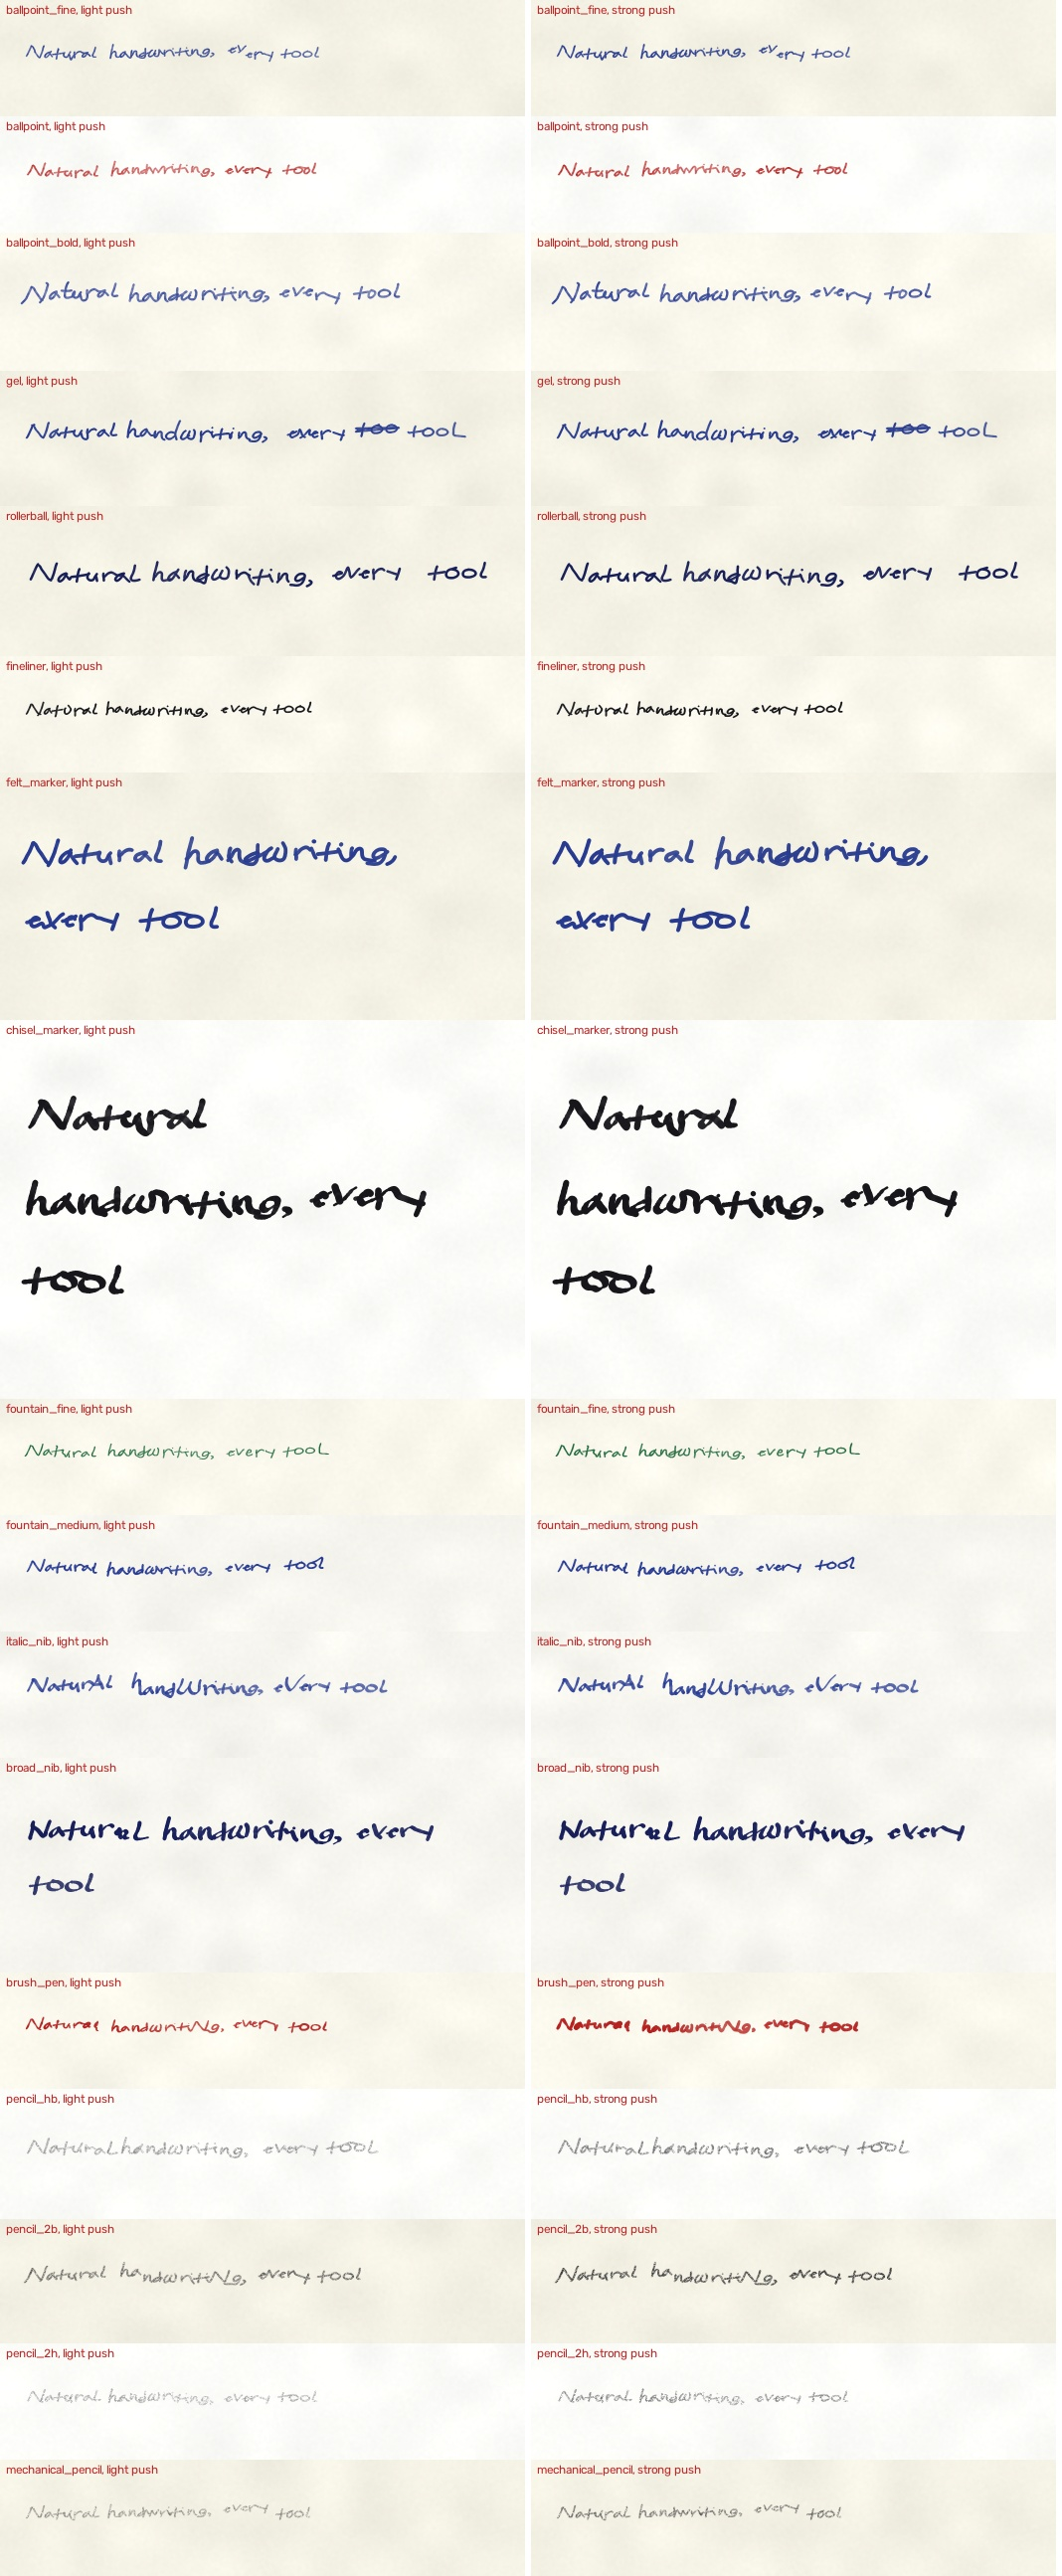
\includegraphics[width=0.95\textwidth,height=0.88\textheight,keepaspectratio]{figs/tools.jpg}
\caption{The 17 tools at light and strong push.}\end{figure}
\clearpage
\begin{figure}[h]\centering
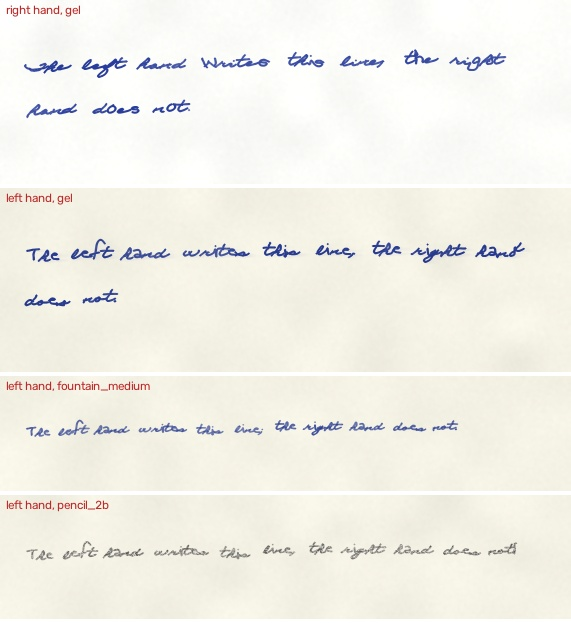
\includegraphics[width=0.95\textwidth,height=0.88\textheight,keepaspectratio]{figs/hands.jpg}
\caption{Right and left hand (gel, fountain pen, pencil): upright slant and smudges.}\end{figure}
\clearpage
